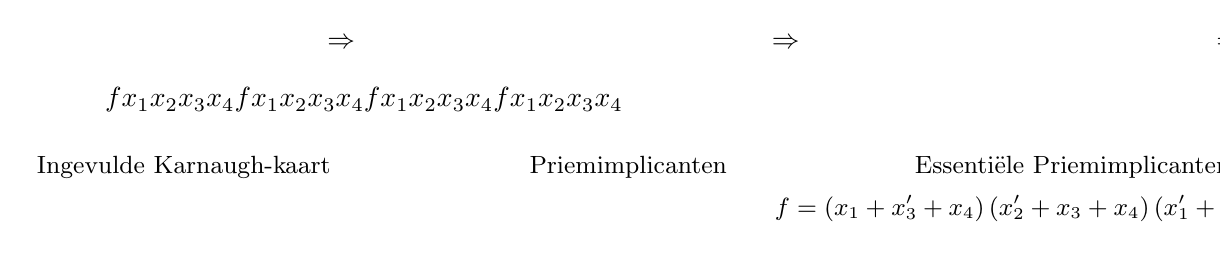
\begin{tikzpicture}
\def\ta{0.09}
\def\tb{0.06}
\draw (1,-0.5) node[anchor=north]{\small{Ingevulde Karnaugh-kaart}};
\draw (3,1) node[anchor=north]{$\Rightarrow$};
\kkaartd{0}{0}{$f$}{$x_1$/$x_2$/$x_3$/$x_4$}{1/1/0/1/0/1/0/1/1/0/1/1/0/0/1/1};
\draw (5,-0.5) node[anchor=north]{\small{Priemimplicanten}};
\draw (7,1) node[anchor=north]{$\Rightarrow$};
\kkaartdmarks{4}{0}{/0/1/1/1/\ta,/1/0/1/1/\tb,/1/0/2/0/\ta,/2/3/3/3/\ta}{}{/2/2/1/\tb};
\kkaartd{4}{0}{$f$}{$x_1$/$x_2$/$x_3$/$x_4$}{1/1/0/1/0/1/0/1/1/0/1/1/0/0/1/1};
\draw (9,-0.5) node[anchor=north]{\small{Essenti\"ele Priemimplicanten}};
\draw (11,1) node[anchor=north]{$\Rightarrow$};
\kkaartdmarks{8}{0}{/0/1/1/1/\ta,/2/3/3/3/\ta}{}{};
\kkaartd{8}{0}{$f$}{$x_1$/$x_2$/$x_3$/$x_4$}{1/1/0/1/0/1/0/1/1/0/1/1/0/0/1/1};
\kkaartdmarks{12}{0}{/0/1/1/1/\ta,/2/3/3/3/\ta,/1/0/2/0/\ta}{}{};
\draw (13,-0.5) node[anchor=north]{\small{Resultaat}};
\draw (7,-1) node[anchor=north]{\small{$f=\left(x_1+x_3'+x_4\right)\left(x_2'+x_3+x_4\right)\left(x_1'+x_3+x_4'\right)$}};
\kkaartd{12}{0}{$f$}{$x_1$/$x_2$/$x_3$/$x_4$}{1/1/0/1/0/1/0/1/1/0/1/1/0/0/1/1};
\end{tikzpicture}